\chapter{Interfaz de usuario}
\label{anexo-e}

A continuación se pueden encontrar más situaciones de ejemplo, además de las presentadas en la \hyperref[section-ui]{seccion 2.4}.\\

En la \hyperref[fig:login-error]{Figura E.1} se puede ver un inicio de sesión en el que se ha producido un error, el cual se recibe del backend y se puede observar también la validación de los campos realizada en el frontend.\\

En la \hyperref[fig:map-carrusel]{Figura E.2} se puede observar la pantalla del plano de alertas con el inicio del carrusel.\\

En la \hyperref[fig:map-presencias]{Figura E.3} se puede ver el ejemplo de que haya presencias.\\

En la \hyperref[fig:list-completa]{Figura E.4} se puede ver la pantalla de lista de alertas completa (la página anterior a la mostrada en la \hyperref[section-ui]{seccion 2.4}).\\


\begin{landscape}
\begin{figure}[!ht]
    \centering
    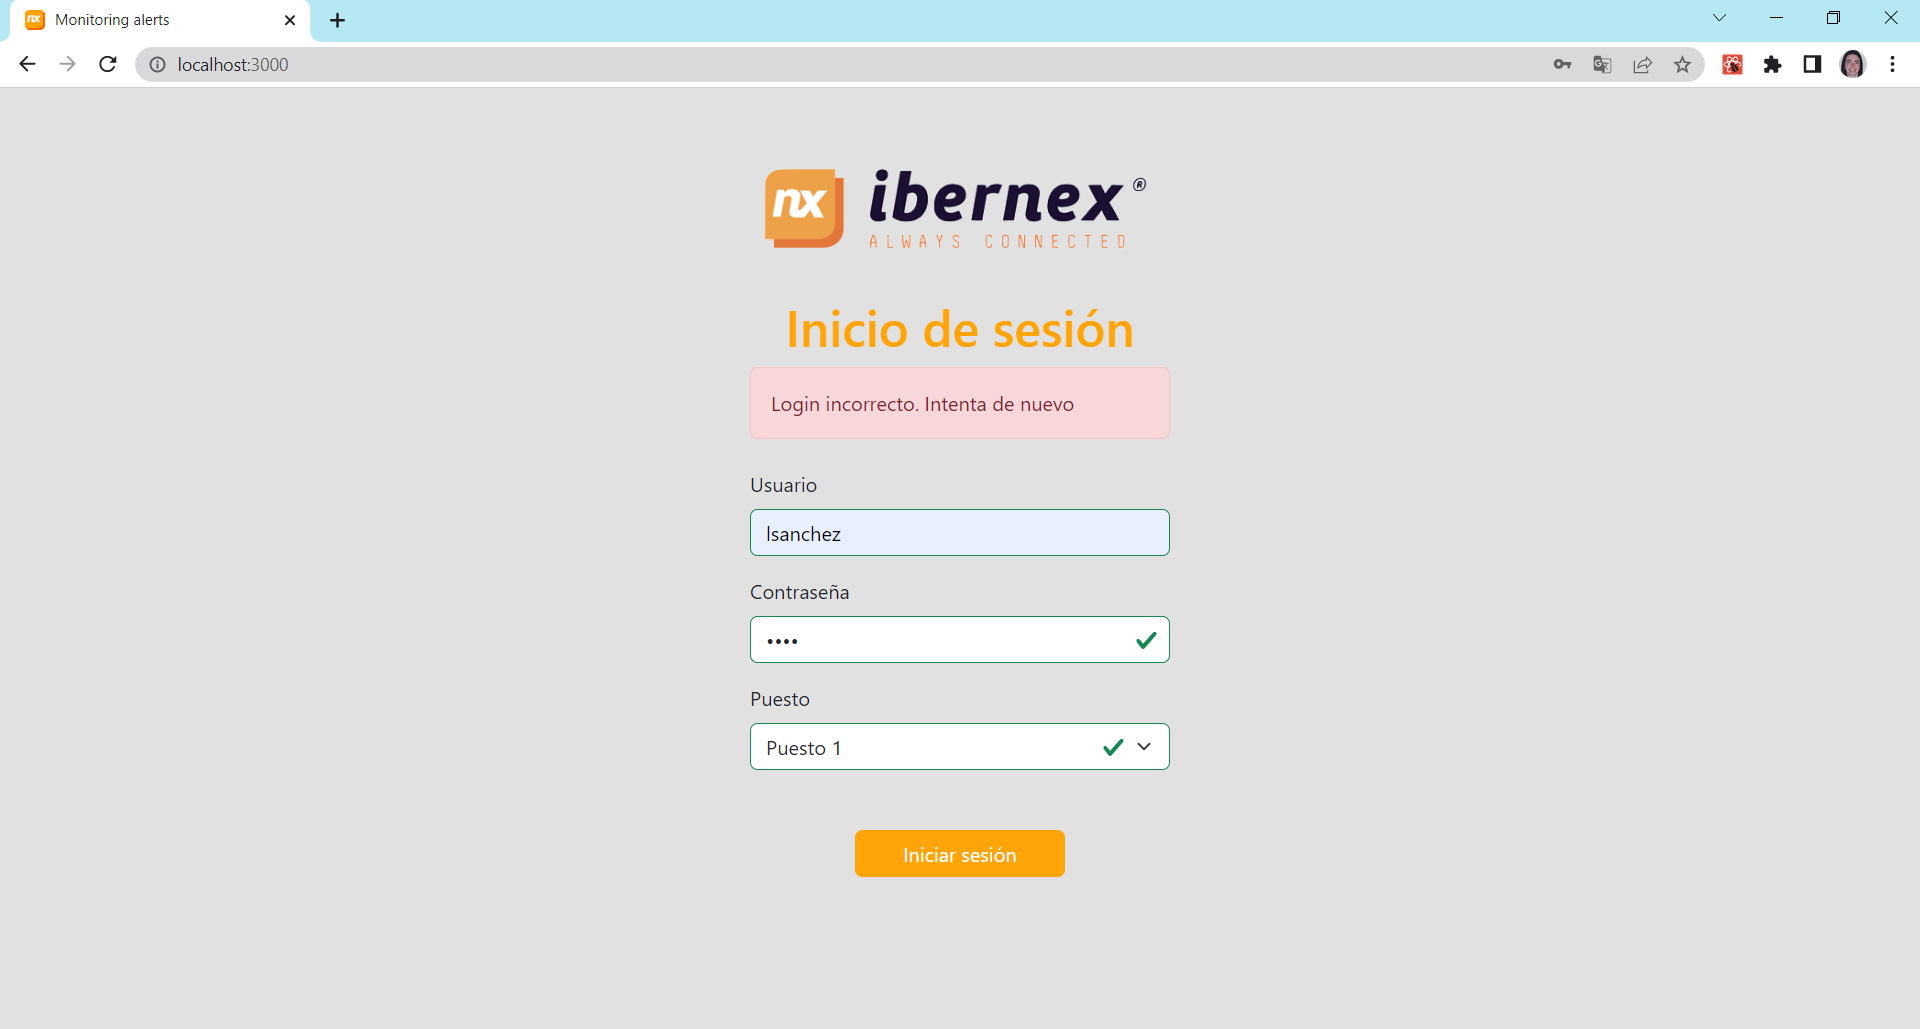
\includegraphics[width=25cm]{Imagenes/login-error.PNG}
    \caption{Pantalla de inicio de sesión con error}
    \label{fig:login-error}
\end{figure}

\begin{figure}[!ht]
    \centering
    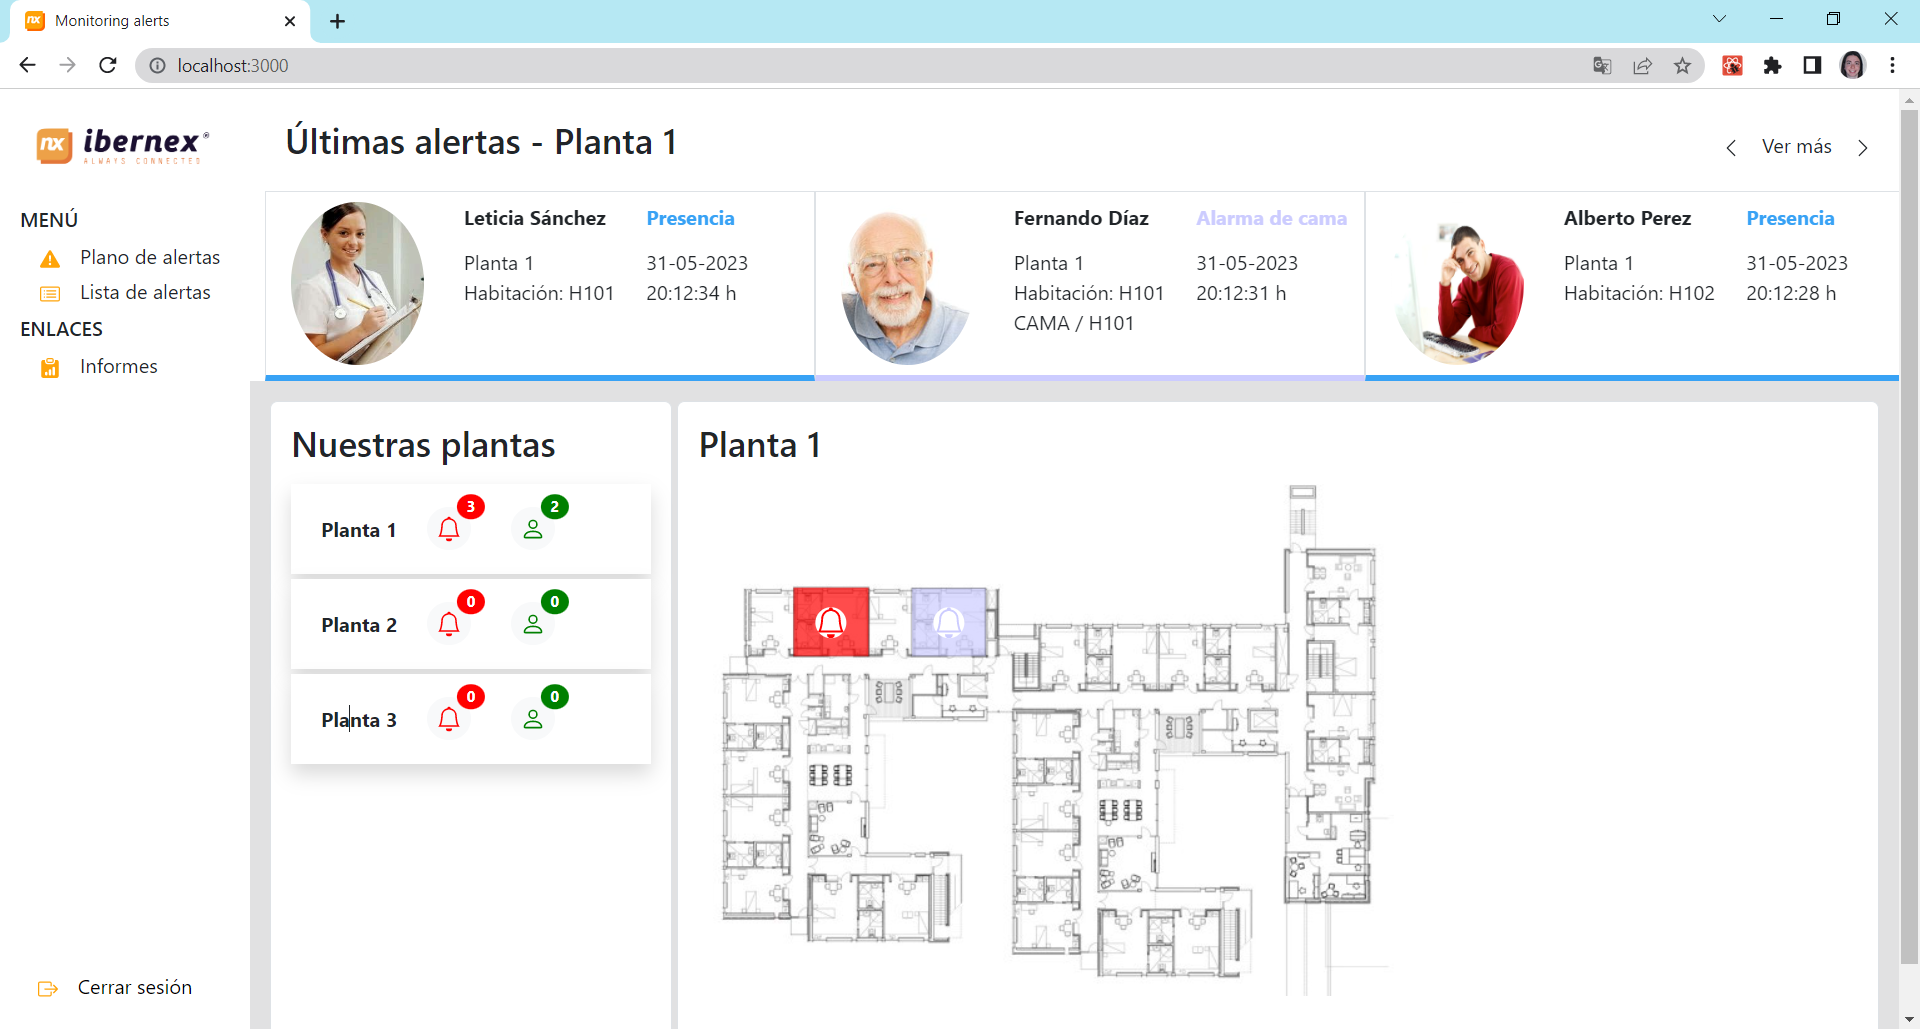
\includegraphics[width=25cm]{Imagenes/map-alarmas-estados-inicio-carrusel.PNG}
    \caption{Pantalla de plano de alertas con inicio de carrusel}
    \label{fig:map-carrusel}
\end{figure}

\begin{figure}[!ht]
    \centering
    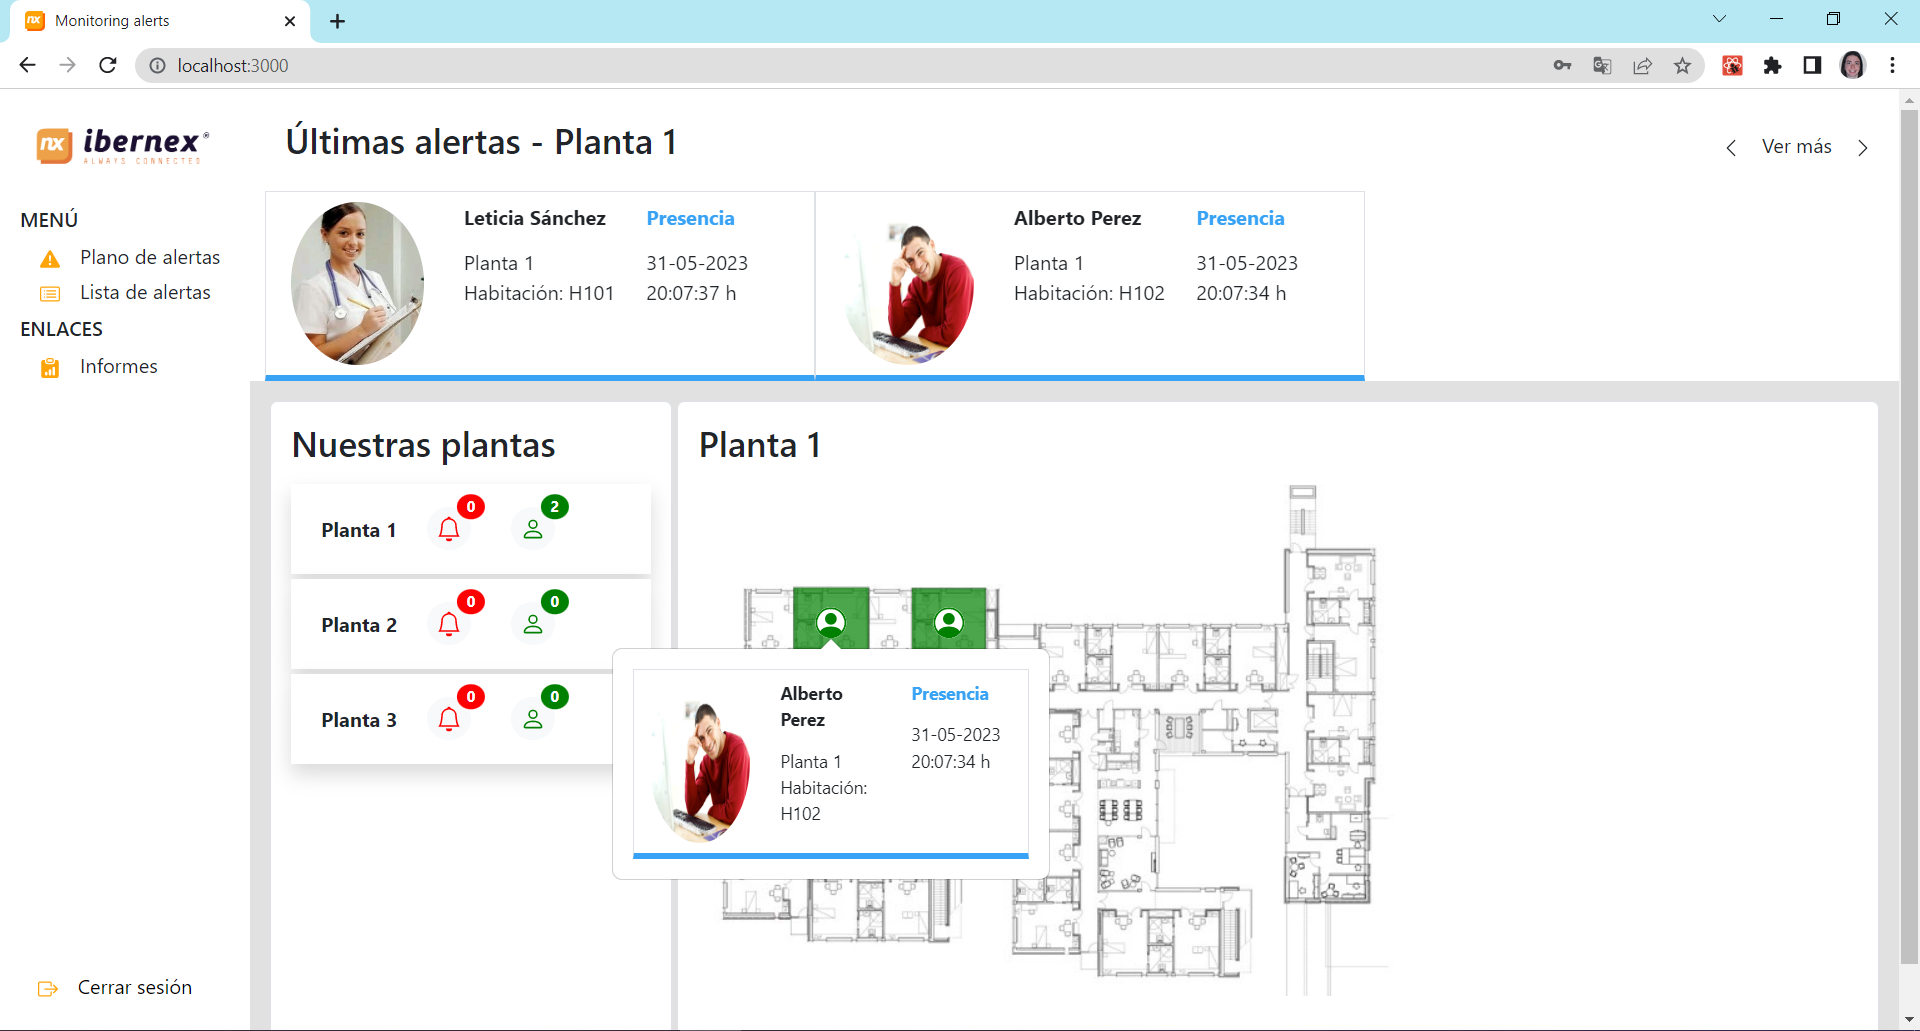
\includegraphics[width=25cm]{Imagenes/map-presencias.PNG}
    \caption{Pantalla de plano de alertas con presencias}
    \label{fig:map-presencias}
\end{figure}

\begin{figure}[!ht]
    \centering
    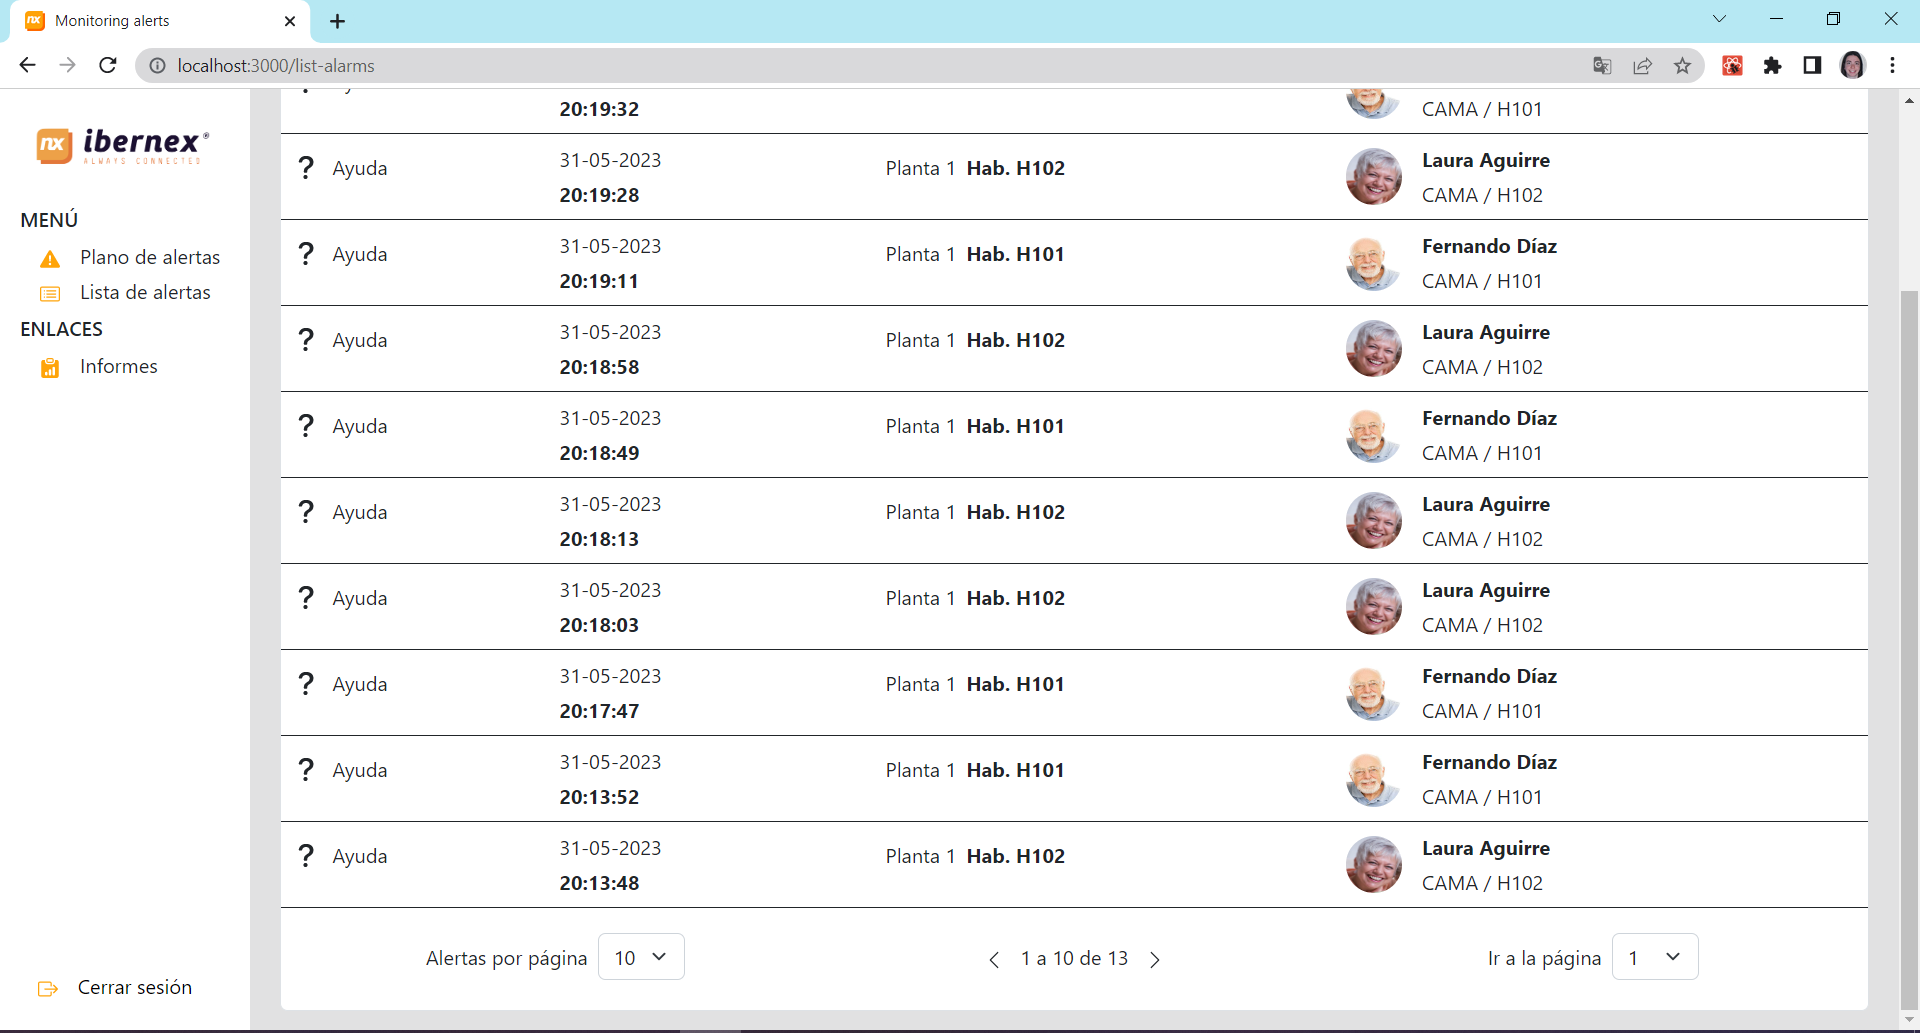
\includegraphics[width=25cm]{Imagenes/list-pag1.PNG}
    \caption{Pantalla de lista de alertas página completa}
    \label{fig:list-completa}
\end{figure}
\end{landscape}